\subsubsection{الگوی \lr{Ordered Locking}}
\label{scheduleOrderedSec}
\begin{RTL}
این الگو نیز برای جلوگیری از بروز \lr{Deadlock} استفاده می‌شود.
روش جلوگیری به این شکل است که منابع را به ترتیبی مرتب می‌کنیم و
کلاینت‌های این منابع را مجبور می‌کنیم که این منابع را به همین ترتیب قفل و
رها کنند. این کار جلوی صبرکردن چرخه‌ای تسک‌ها برای یکدیگر را می‌گیرد.
\end{RTL}
\begin{figure}[h!]
\centering
\begin{tikzpicture}
    \lr{
        \umlclass[x=-1]{ResourceClient}{
            \lr{}
        }{}
            \umlclass[x=3, y=-4]{OrderedResource}{
            \lr{resourceID}
        }{
            \lr{monadicAccessFunction()}\\
            \lr{dyadicAccessFunction()}\\
            \lr{lockDyadic()}\\
            \lr{releaseDyadic()}
            }
            \umlclass[x=3, y=-10]{ResouceList}{
                \lr{}
            }{
                \lr{islnOrder()}\\
                \lr{addLock()}\\
                \lr{removeLock()}
                }
                \umlclass[x=9, y=-7.5]{Mutex}{
                    \lr{mutexID}
                }{
                    \lr{lock()}\\
                    \lr{release()}
                }    
    \umlclass[x=3, y=-15]{ResouceRefrence}{
    \lr{resourceID}
}{
    \lr{}
}    
    \umluniassoc[mult2=1, geometry=-|, pos2=1.7]{OrderedResource}{Mutex}
    \umluniassoc[mult2=*, geometry=|-, pos2=1.6]{ResourceClient}{OrderedResource}
    \umluniassoc[mult2=1]{OrderedResource}{ResouceList}
    \umluniassoc[mult2=1, geometry=-|, pos=1.7]{ResouceList}{Mutex}
    \umluniaggreg[attr2=*|\{ordered\}]{ResouceList}{ResouceRefrence}
    }
\end{tikzpicture}
\caption{دیاگرام کلاس \lr{Ordered Locking}}
\label{scheduleOrderedClassDiag}
\end{figure}
\begin{RTL}
همانطور که در شکل \ref{scheduleOrderedClassDiag} دیده
می‌شود، در این ساختار، کلاینت باید برای استفاده از منابع، از کلاس
\lr{OrderedResource} استفاده کند. این کلاس می‌تواند منابع را به
دو فرم \lr{monadic} و \lr{dyadic} در اختیار او قرار دهد.
این کلاس با مدیریت منابع، این اطمینان را ایجاد می‌کند که ترتیب قفل‌شدن
و آزادسازی منابع، طبق ترتیبی که از پیش بر اساس \lr{resourceID}
تنظیم‌شده انجام می‌شود.
\end{RTL}